\documentclass[modern]{aastex61}

\newcommand{\escapecmd}[1]{\texttt{\detokenize{#1}}}

\submitjournal{ApJ}

\shorttitle{Astropy Project II}
\shortauthors{Astropy Project et al.}

\begin{document}

\draft{\today}

\title{The Astropy Project: }

\correspondingauthor{Astropy coordination committee}
\email{coordinators@astropy.org}

\author{Astropy Collaboration}

\begin{abstract}
The Astropy project supports and fosters the development of open-source Python
packages that provide commonly-needed functionality to the astronomical
community.
A key element of the project is the Astropy core package, which serves as the
foundation for more specialized projects and packages.
In this article, we provide an overview of the organization of the Astropy
project and summarize key features in the core package as of the recent major
release, version 2.0.
We then describe the project infrastructure designed to facilitate [...]
We conclude with a future outlook of planned new features and directions for the
broader Astropy ecosystem.
\end{abstract}

%% Keywords should appear after the \end{abstract} command.
%% See the online documentation for the full list of available subject
%% keywords and the rules for their use.
\keywords{}

\section*{\textit{Notes and guidelines (to be removed)}}

\begin{itemize}
   \item The goal is to produce a brief and informative paper that covers major astropy principles not mentioned in the first paper, the core v2.0 package, and infrastructure in astropy project to support development in python.   
	\item We don't plan on including code in this paper, but if you think you will need to include code in your section, please add it to a separate Python module (.py file) and include it in this repository.
    \item Use \escapecmd{\sectionname} not ``Section,'' \escapecmd{\figurename} not ``Figure''
    \item If your subpackage was included in Paper I, then please just include a note on what the package does, a reference to paper I, and any new major updates to your package
    \item If your subpackage was not included, then please a further description of the sub-package on level with what was in the first paper, and highlight any major features in it.   Typically length should be equivalent to one column
    \item Please make sure you are logged into Overleaf or pushing a commit with your information to be able to track the contributors to the paper. 
    
\end{itemize}

\section{Introduction} \label{sec:intro}
% Moritz (first draft)


\section{Major concepts}
% Anyone want to take this??

\subsection{Astropy development model, astropy ecosystem}
This subsection should include some basic statistics about the contributors, commits, line of code etc. up to the 2.0 release when we know it.

\subsection{Mixin}

\subsection{Accuracy testing across many different implementation}

\subsection{Use of Quantities across package}
% Marten and Tom R. 

{\bf Very rough first text!}

Historically, it has been unusual to keep units as part of numbers, especially as speed was often deemed essential and quantities used to be slower than regular arrays. Hence, programs and functions expected to be fed parameters in particular units, as (hopefully) stated in their documentation.  In astropy 0.4, therefore, unit and quantity support was still somewhat spotty, but this has changed greatly.  One of the riskiest classes was ngles, where both degrees and radians were ``obvious'' default units to some. As a consequence, quantities are most fully integrated in the coordinates module (Sect.~\ref{sec:coordinates}). In astropy 2.0, one can also opt in to use quantities fully in tables, by using the {\tt QTable} class (see Sect.~\ref{sec:table}). As a result, units in fits tables are also well-supported. For most other modules, quantities are at least accepted, and often assumed by default.

In the process, some standard wrappers have been defined that make defining functions that require quantities as input simpler. As an extension of this, we plan to define wrappers for functions that work on numbers that will automatically convert quantities to any required units.

\subsection{Long term support of v2.0}
% This could also include information about the development cycle

%\subsection{Difficulty of reversing design choices}
%Deciding if a feature should be included
%difficulty to decide where general use ends and "handy feature for some" starts, i.e. how to reject PRs or deal with maintenance burden

\section{Astropy Core Package v2.0}

The astropy project aims to provide python-based packages for all tasks that are commonly needed in a large subset of the astronomical community. Two aspects of this (time and coordinate transformations) are already discussed in great detail in section 3. In this section, we highlight other features introduced or substantially improved since version v0.2, which is described in \citet{2013A&A...558A..33A}.
(ordered in the order in which they appear in the astropy documentation)

% \subsection{Analytic Functions}
% moved to models and depreciated -- 
% just here for completeness at the moment

\subsection{Units and quantities}
\label{sec:units}
% Marten, Adrian

\textbf{Key features:}
\begin{itemize}
	\item incl logarithmic units and magnitudes
	\item speed improvements
    \item interaction with numpy arrays
\end{itemize}

\subsection{Constants}
% David S.
versioning


\subsection{Coordinates}
\label{sec:coordinates}
% Adrian, Erik

The \texttt{astropy.coordinates} subpackage is designed to support representing
and transforming celestial coordinates and velocities.


- Three-tiered structure for coordinates: representation, frame, skycoord
- With differential classes, frames support velocities

Accuracy and comparison of coordinate system definitions?

\textbf{Key features:}
\begin{itemize}
	\item Celestial coordinates, and local coordinates (via EarthLocation + Time)
	\item JPL ephemerids
    \item Proper motions, radial velocities
\end{itemize}

Separately, talk about representations as vectors? (MHvK)

\subsection{Time}
\label{sec:time}

Q: does it make sense to refer forward to fits support, even though it is 3.0?

\subsection{Data arrays}

\subsubsection{NDDdata}
% Matt C., Michael, or Steve C.
% Larry (nddata.utils)
NOTE (Larry), The package is nddata, which includes the NDData object.  Don't forget the nddata.utils functionality (e.g. Cutout2D, block\_reduce, etc.).

\subsubsection{Tables}
\label{sec:table}
% Tom A.
QTable is new, mixin columns for time and coordinates. Table operations were added in v0.3

\subsection{io}
% Simon



\subsection{Modeling}
\label{sec:modeling}
% Nadia
% Lim blackbody
% Tom R. -- unit support
The whole modeling submodule was missing from the previous paper, so everything really, including compound models, unit support etc.

\subsection{Convolution}
% Adam G.

Astropy implements `normalized convolution' \citep[e.g.,][]{Knutsson1993}, which is an image reconstruction technique in which missing data are ignored during the convolution and replaced with values interpolated using the kernel.   In version $<=1.3$, the direct convolution and fft convolution approaches were not consistent, with fft convolution implementing normalized convolution and direct convolution implementing a different approach.  As of v2.0, the two methods are consistent and include a suite of consistency checks.


\begin{figure}
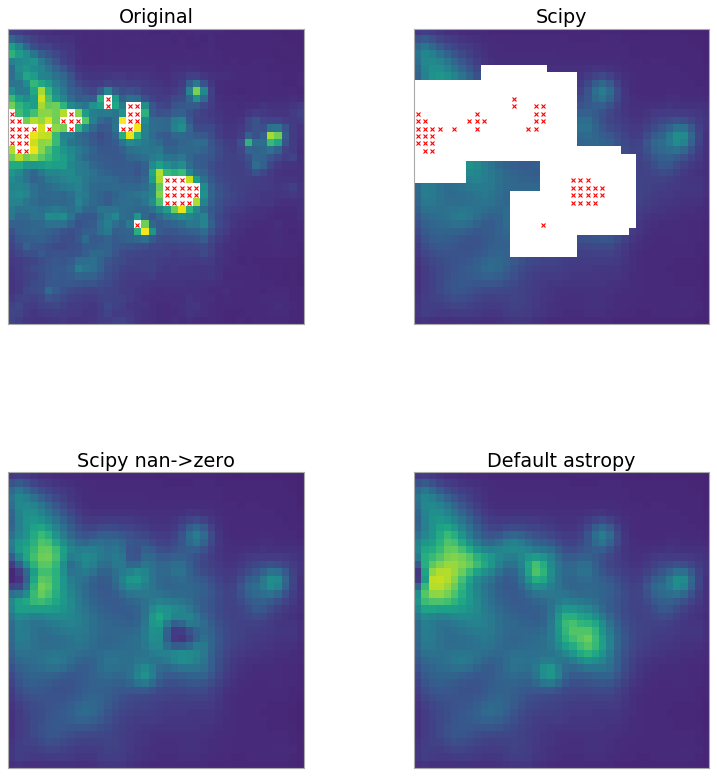
\includegraphics[width=\textwidth]{convolution_example.png}
An example showing different modes of convolution available in the python ecosystem.  The red x's mark pixels that are set to NaN in the original data (a).  If the data are convolved with a Gaussian kernel on a 9x9 grid using scipy's direct convolution (b), any pixel within range of the original NaN pixels is also set to NaN.  Panel (c) shows what happens if the NaNs are set to zero first: the originally NaN regions are depressed relative to their surroundings.  Finally, panel (d) shows astropy's convolution behavior, where the missing pixels are replaced with values interpolated from their surroundings using the convolution kernel.
\end{figure}


\subsection{Visualization}
% Larry:  Image visualization (stretching, scaling), RGB
% Tom R.:  WCSAxes

wcsaxis, rgb, histograms comes to mind.Can use more publicity and also makes good images to include in the paper.


%\subsection{Utils}
% Lim 

\subsection{Cosmology}


\subsection{Statistics}
% Steve C.
% Jake V.:  Lomb-scargle, Bayesian blocks
% Larry:  sigma clipping, biweight stats
major additions to be discussed: lomb-scargle, sigma clipping, bayesian blocks, histograms, also:  robust (biweight) statistics

\section{Infrastructure for affiliated packages}
\subsubsection{Package template}
bsipocz may write this up if there is no other takers
\subsection{Continuous integration helpers}
bsipocz should write this up
\subsection{sphinx extensions}
probably Tom R should write this up


% \section{State of the Ecosystem}
% Commenting out unless a clear statement is added 

\section{Learning Astropy}
% Kelle, Adrian

Explain components: Documentation, Example gallery, Tutorials and lessons

\section{The future of the Astropy project}

dropping python2 support, growths of affiliated packages
Summary

\acknowledgments

Who to thank?  numfocus, 

%% Similar to \facility{}, there is the optional \software command to allow
%% authors a place to specify which programs were used during the creation of
%% the manusscript. Authors should list each code and include either a
%% citation or url to the code inside ()s when available.

\software{astropy \citep{2013A&A...558A..33A},
          numpy,
          scipy,
          }

\bibliographystyle{aasjournal}
\bibliography{bibliography}

\begin{thebibliography}{}

\end{thebibliography}



\end{document}

